\documentclass{article}

\usepackage{polski}
\usepackage[utf8]{inputenc}
\usepackage[ruled,vlined]{algorithm2e}
\usepackage{indentfirst}
\usepackage{amssymb}
\usepackage[colorlinks=true]{hyperref}
\usepackage[margin=1.3in]{geometry}
\usepackage{physics}

\usepackage{graphicx}
\usepackage{float}
\graphicspath{ {./images/} }

\usepackage[backend=biber]{biblatex}
\addbibresource{bibliography.bib}

\usepackage{amsmath}
\renewcommand{\vec}[1]{\mathbf{#1}}

\title{GA \& DNN}
\author{Jan Sołtysik}


\begin{document}
\maketitle
\tableofcontents


\section{Wstęp}
W ostatnich latach sieci neuronowe i uczenie głębokie  są tematem numer jeden w świeci
informatyki. Jest to jednak stosunkowo stara dyscyplina ponieważ jej początek sięga roku 1943 
w którym został zaprezentowany model pojedynczego perceptronu.\\
Jednak dopiero w latach dwutysięcznych zaczęła ona pokazywać swój prawdziwy potencjał.
Przyczyniło się do tego wiele czynników m.in. rozwój technologi, ogólnodostępne duże pokłady
danych itd. Wiele firm  zaczyna to wykorzystawać wprowadzając różnego 
rodzaju zastosowania dla SSN np. Tesla i samoprowadzące się samochody, system rekomendacji 
filmów na platformie Netflix, filtry spam w skrzynkach e-mail, boty uczącę się grać w gry
z OpenAI  i wiele wiele innych.\\
Zbudowanie jednak sieci składającej się z dużej ilości warstw nie jest jednak proste. 
Dlatego zaczęto opracowywać metody automatycznego budowania sieci neuronowych. 
Metody te umożliwiają osobom niezaznajomionym z uczeniem maszynowym na korzystanie z SSN. Jednym
z możliwych podjeść są Algorytmy Genetyczne, które podobnie jak SSN nie są wynalazkiem
ostatnich lat (rok 1960 John Holland). Znajdują one jednak wciąż nowe zastosowania.\\
Tematem tej pracy będzie implementacja Algorytmu Genetycznego w celu znalezienia optymalnej
struktury sieci neuronowej.


\section{Wprowadzenie teoretyczne}

\subsection{Algorytm Genetyczny}
Algorytmy genetyczne są to algorytmy poszukiwania zainspirowane mechanizmem doboru naturalnego
oraz dziedziczności. Łączą w sobie  zasadę przeżycia najlepiej przystosowanych 
osobników z systematyczną, choć zrandomizowaną wymianą informacji wprowadzoną przez
operatory genetyczne takie jak krzyżowanie i mutacja, które również zainspirowane są
przyrodą. W każdym pokoleniu powstaje
nowy zespół sztucznych organizmów, utworzonych z połączenia fragmentów najlepiej przystosowanych
przedstawicieli poprzedniego pokolenia. Oprócz tego sporadycznie wyporóbowuje się nową część 
składową. Element losowości nie oznacza że algorytmy genetyczne sprowadzają się do zwykłego
błądzenia przypadkowego. Dzięki wykorzystaniu przeszłych doświadczeń algorytm określa nowy obszar
poszukiwań o spodziewanej podwyższonej wydajności.
Algorytm genetyczny jest przykładem procedury używającej wyboru losowego jako 
"przewodnika" w wysoce ukierunkowanym poszukiwaniu w zakodowanej przestrzeni rozwiązań
\cite{goldberg}.\\

Poniżej znajduję się podstawowy algorytm genetyczny przedstawiony w postaci
pseudokodu \cite{ams}:\\
\begin{algorithm}[H]
 \SetAlgoLined
 \KwIn{Funkcja oceny $f(\vec{x})$}
 \KwData{$\vec{x}_i(t)$ - $i$-ty osobnik z generacji nr. $t$(najczęściej reprezentowany jako
 	 ciąg znaków), $n_x$ - wymiar każdego osobnika}
 \KwOut{Wektor $\hat{\vec{x}}$ dla którego $f(\hat{\vec{x}})$ jest lokalnym minimum}
 Niech $t = 0$ będzie licznikiem generacji. 
 Wygeneruj $n_x$ - wymiarową populację $\mathcal{C}(0)$, składającą się z n osobników.\\
 \While{Warunek końcowy nie jest prawdziwy}{
	Oblicz przystosowanie, $f(\vec{x}_i(t))$ każdego osobnika $\vec{x}_i(t)$ z populacji.\\
	W celu stworzenia potomstwa do najlepiej przystosowanych osobników zastosuj operatory
	genetyczne np. krzyżowanie i mutacja.\\
	Z nowo powstałych osobników stwórz nową populację $\mathcal{C}(t + 1)$.\\
	Przejdź do nowej generacji. $t = t + 1$.\\
 }
 \caption{\label{alg:ag}Podstawowy Algorytm genetyczny}
\end{algorithm}

\subsubsection{Podstawowa reprezentacja}
Jednym z następstw inspiracji biologicznych AG jest słownictwo zaczerpnięte 
z genetyki którym będę się posługiwać w tej pracy.
\textbf{Fenotypem} nazywamy  układ złożony z pewnej liczby parametrów opisujących cechy
rozwiązania. 
Osobniki występujące w populacji nazywane są \textbf{genotypami}, które 
składają się z zakodowanej wersji opisanych dla fenotypu parametrów. 
Konkretna zakodowana cecha (parametr) nazywana jest \textbf{genem}. Każdy gen może przyjmować 
różne wartości, które nazywane są \textbf{allelami}. Pozycję na jakiej znajduję się gen nazywamy
\textbf{locusem}. \textbf{Chromosomem} nazywamy uporządkowanym zestawem genów.
Opisany wyżej genotyp składa się z jednego lub więcej genotypów.\cite{goldberg}.

Poniższa tabela przedstawia używane przeze mnie odpowiedniki:
\begin{table}[H]
\centering
\begin{tabular}{|c|c|}
	\hline
	Genetyka & Algorytmy Genetyczne\\
	\hline
	genotyp & osobnik w populacji\\
	gen & składowe osobnika\\
	allel & możliwe warianty składowych\\
	locus & pozycja składowej\\
	chromosom & struktura złożona z składowych\\
	\hline
\end{tabular}
\caption{\label{tab:ag}Słownictwo używane w AG.}
\end{table}

W elementarnym AG \textbf{genotyp} reprezentujemy za pomocą ciągów bitów, więc \textbf{genami}
będą pojedyncze bity.
Poniżej znajduję się przykładowy genotyp:\\

\begin{figure}[H]
\centering
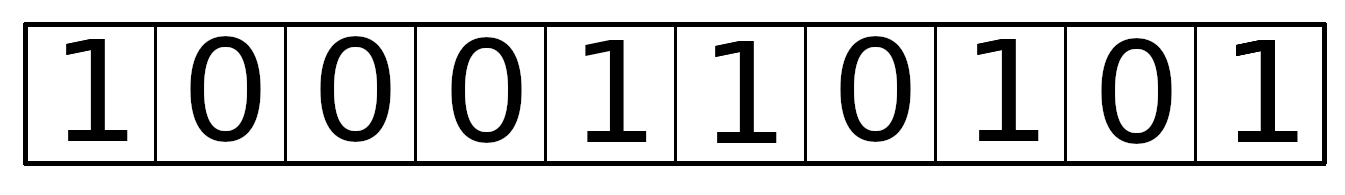
\includegraphics[scale=0.20]{genome_v2.png}
\caption{Przykładowy genotyp o długości 10.}
\end{figure}

Transformacja naszego problemu do opisu w postaci ciągów binarnych jest często bardzo trudna, a
czasami wręcz niemożliwa. Lecz trud ten jest opłacalny, ponieważ dla tak opisanych genotypów mamy
zdefiniowane operatory genetyczne, które wykonując proste obliczenia zbliżają nasze osobniki do
optymalnego rozwiązania.

\subsubsection{Selekcja}
Selekcja jest to etap algorytmu w którym wybieramy poszczególne genotypy które później zostaną 
poddane operatorom genetycznym. Celem tej operacji jest wybranie najlepiej przystosowanych
osobników do utworzenia nowej populacji.
Aby opisać ten proces musimy zdefiniować przedstawioną w [\hyperref[alg:ag]{Alg. 1}]
funkcję oceny $f$.\\
\textbf{Funkcja oceny/przystosowania} $f$ jest obliczana dla każdego osobnika i pozwala nam
porównać które genotypy są najlepiej przystosowane do zadania które optymalizujemy.\\
Najprostszym przykładem będzie zadanie znalezienia maximum funkcji 
$f(x_1, ..., x_n)$ gdzie $n \in \mathbb{N}^{+}$, wtedy funkcja przystosowania
będzie równa wartości funkcji $f$, im większa wartość $f$ tym osobnik jest
lepiej przystosowany.\\\\
W prostym AG wszystkie genotypy poddawane są reprodukcji, lecz w ogólnym przypadku przy pomocy
funkcji oceny i różnych metod selekcji wybierana jest pula "najlepszych osobników".
Istnieje wiele metod selekcji lecz zdecydowanie najpopularniejszą jest \textbf{metoda ruletki}
w której prawdopodobieństwo $p_i$
wybrania $i$-tego genotypu do reprodukcji kolejnego pokolenia jest proporcjonalne do wartości
funkcji przystosowania. Prawdopodobieństwo to jest równe:\\
\begin{equation}
	p_i = \frac{f_i}{\sum_{j=1}^{N} f_j}
\end{equation}
gdzie:\\
$f_i$ - wartość funkcji oceny dla $i$-tego genotypu, $N$ - rozmiar populacji.\\

\subsubsection{Krzyżowanie}
Jedną z dwóch podstawowych operacji wykonywanych w celu stworzenia potomstwa obecnej populacji
jest \textbf{krzyżowanie}, które inspiruję się rozmnażaniem płciowym w biologi \cite{cross}.

W literaturze możemy znaleźć wiele rodzajów tej operacji, poniżej znajdują się najpopularniejsze
odmiany:
\begin{itemize}
\item \textbf{Krzyżowanie jednopunktowe}:\\
W tej odmianie potomka tworzymy z dwóch wybranych przez selekcję rodziców a następnie 
losujemy liczbę naturalną  $l$ ze zbioru $\{1,\ldots, n_x\}$.
Potomek wartości na pierwszych $l$ pozycjach przyjmuje wartości od pierwszego rodzica
a na pozostałych od drugiego.
\begin{figure}[H]
\centering
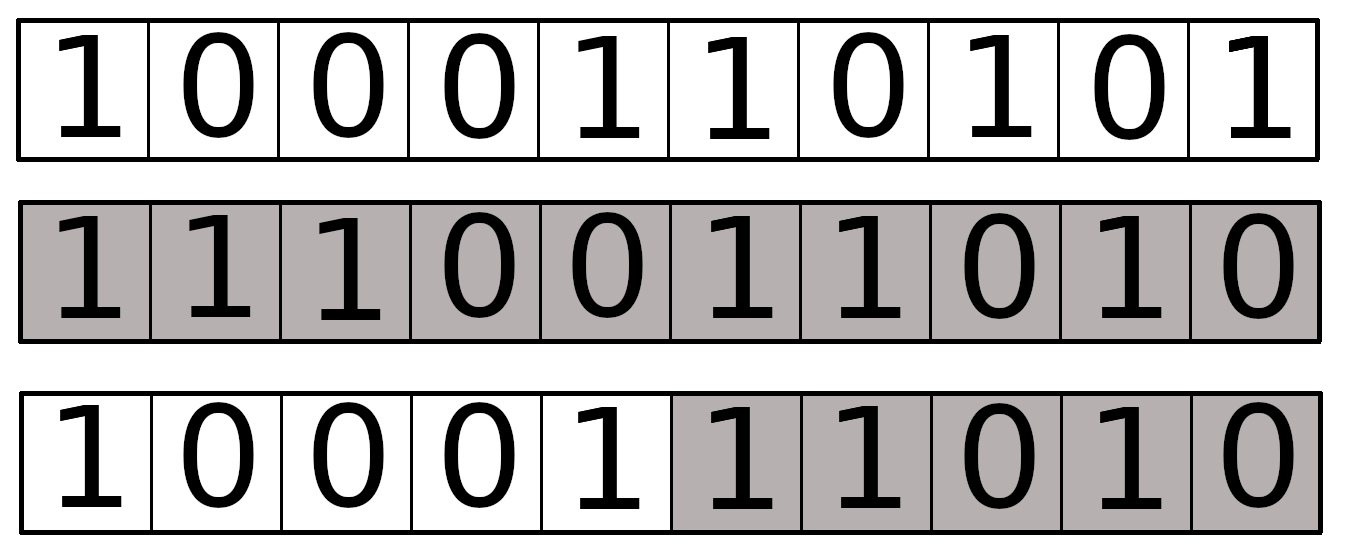
\includegraphics[scale=0.2]{crossover_v2.png}
\caption{Krzyżowanie jednopunktowe, gdzie $n_x = 10$ i $l = 5$.}
\end{figure}

\item \textbf{Krzyżowanie dwupunktowe}:\\
Sposób ten jest zbliżony do opisanego wyżej lecz zamiast jednego punktu losujemy dwie liczby
naturalne $l_1, l_2$ ze zbioru $\{1,\ldots, n_x\}$, gdzie $l_1 < l_2$.
Potomek natomiast przyjmuje wartości z pierwszego rodzica poza elementami na pozycjach od
$l_1$ do $l_2$ gdzie wstawiamy elementy z drugiego.

\begin{figure}[H]
\centering
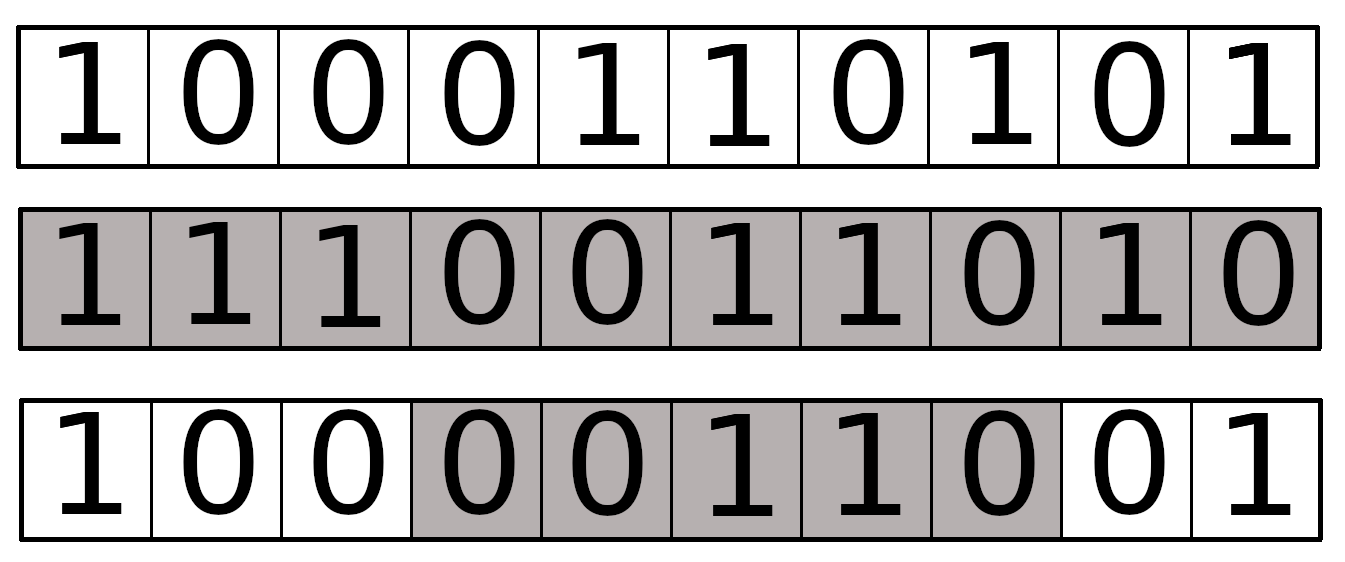
\includegraphics[scale=0.2]{two_crossover_v2.png}
\caption{Krzyżowanie dwupunktowe, gdzie $n_x = 10$, $l_1 = 4$ i $l_2 = 8$.}
\end{figure}

Krzyżowania tego rodzaju można uogólnić na operacje gdzie losujemy k-punktów
a potomek naprzemiennie pobiera wartości z rodziców.\\
\item \textbf{Krzyżowanie równomierne}:\\
Potomek jest również tworzony przy pomocy dwóch rodziców gdzie każdy jego element jest
wybierany losowo z pierwszego lub drugiego rodzica z jednakowym prawdopodobieństwem 
(lub wybranym innym stosunkiem prawdopodobieństw).

\end{itemize}

\subsubsection{Mutacja}
Operator ten w klasycznej wersji algorytmu polega na zamianie zadanej wartości bitu
(0 na 1 lub 1 na 0) z bardzo małym  prawdopodobieństwem $\sigma_m$(np. 0.02\%).
\begin{figure}[H]
\centering
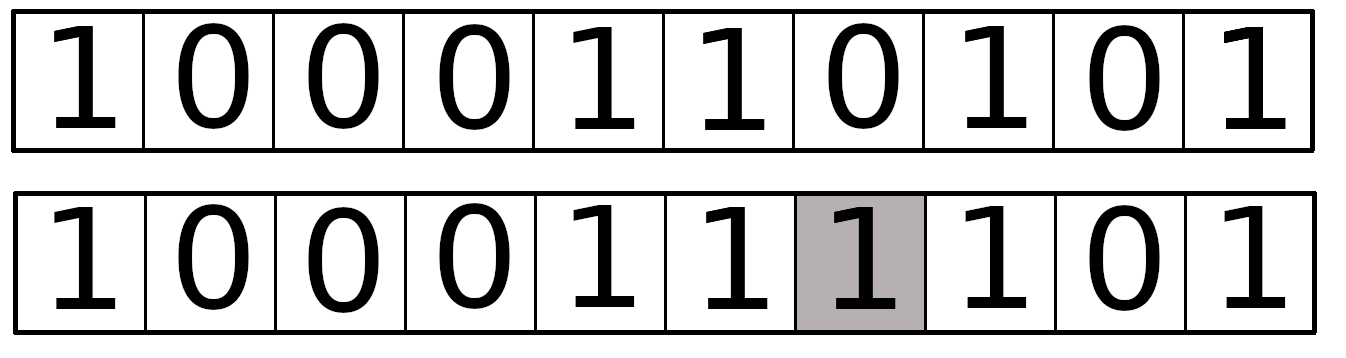
\includegraphics[scale=0.2]{mutation_v2.png}
\caption{Podstawowa mutacja dla genotypu o $n_x = 10$ i wylosowanej pozycji 7.}
\end{figure}



\subsection{Sztuczne Sieci Neuronowe}
\label{sec:ssn}
Podobnie jak dla Algorytmów Genetycznych, inspiracją dla Sztucznych Sieci Neuronowych (SSN) 
była biologia a dokładniej budowa neuronów naturalnych znajdujących się w ciele człowieka.
Sztuczne sieci neuronowe zostały wymyślone już w w pierwszej połowie XX wieku, lecz dopiero w ostatnich latach
dzięki rozwojowi technologi oraz dostępności do olbrzymiej ilości danych mogliśmy zacząć używać
ich pełny potencjał. SSN są przykładem techniki \textbf{uczenia nadzorowanego} tzn.
podczas uczenia sieci podajemy mu dane ze znanymi wynikami i poprzez porównywanie wygenerowanych
wyników z rzeczywistymi nasza sieć uczy się generować poprawne wyniki.

\subsubsection{Perceptron}
\textbf{Perceptron} to  najprostsza architektura SSN. Jednostki na wyjściach/wejściach
nazywane są \textbf{neuronami}. Na neuronach wejściowych  podawane są liczby oraz
każde połączenie ma przypisaną  wagę natomiast $j$-te wyjście perceptronu jest obliczane przez 
wyliczenie ważonej sumy sygnałów wejściowych:
\begin{equation}
	z = \sum_{i=1}^n w_{ij}x_i = \vec{w}^T\vec{x}
\end{equation}
gdzie:\\
$w_{ij}$ - waga połączenia pomiędzy $i$-tym neuronem wejściowym a $j$-tym wyjściowym,\\
$x_i$ - $i$-ta wartość wejściowa.\\ \\
Następnie wynik otrzymany w (2) jest poddawany \textbf{funkcji skoku}, gdzie najczęściej jest 
ona równa \textbf{funkcji Hraviside'a} lub \textbf{signum} które są równe:
\[
	\text{Heaviside}(z) = \
	\begin{cases}
		0, \: z < 0 \\
		1, \: z \geq 0
	\end{cases} 
	\text{sgn}(z) = \
	\begin{cases}
		-1, \: z < 0 \\
		0, \: z = 0 \\
		1, \: z > 0
	\end{cases} 
\]
Nazywane są one \textbf{funkcjami aktywacji} (patrz [\hyperref[sec:fa]{2.2.3}])
i jest to jeden z wielu hiperametrów SSN które samodzielnie musimy wybrać podczas
tworzenia sieci.\\

\begin{figure}[H]
\centering
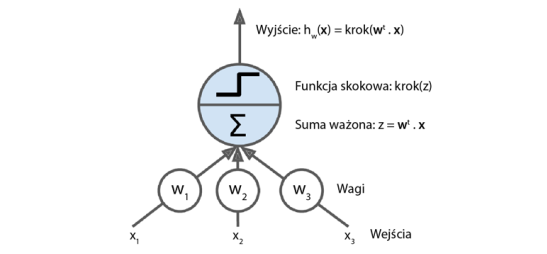
\includegraphics[scale=0.5]{perceptron.png}
\caption{Schemat perceptronu z jednym neuronem wyjściowym i trzema wejściowymi \cite{um}}
\end{figure}

Lecz aby na wyjściu otrzymywać oczekiwane wyniki musimy najpierw perceptron wytrenować. Proces
ten polega na modyfikacji wag na podstawie porównania wyniku oczekiwanego z wynikiem otrzymanym.
Wagi są aktualizowane według wzoru \cite{um}:
\begin{equation}
	w_{ij} = w_{ij} + \eta(y_j - \hat{y_j})x_i
\end{equation}
gdzie:\\
$\hat{y_j}$ - otrzymany wynik na $j$-tym wyjściu,\\
$y_j$ - docelowy wynik $j$-tego wyjścia,\\
$\eta \in$ (0, 1] - współczynnik uczenia.\\
Perceptron jednak nie nadaje się do skomplikowanych zadań ponieważ przez swoją prostą budowę
jest jedynie zdolny do klasyfikowania danych które są liniowo separowalne.

\subsubsection{Wielowarstwowa Sieć Neuronowa}
Ograniczenia perceptronu można wyeliminować tworząc SSN z wielu warstw perceptronów.
SSN tego typu nazywamy \textbf{perceptronem wielowarstwowym}, który jest złożony z 
\textbf{warstwy wejściowej}, co najmniej jednej \textbf{warstwy ukrytej} (jako wejście przyjmują
one wyjście poprzedniej warstwy a ich wyjście propagowane do kolejnej jako wejście) ostatnią
warstwę nazywamy \textbf{warstwą wyjściową}. Dodatkowo w każdej warstwie znajduję się 
\textbf{neuron obciążający}, którego zadaniem jest wysyłanie na wejście następnej warstwy 
wartości 1. Ilość neuronów w warstwie wejściowej i wyjściowej jest określana przez
zestaw danych na których sieć ma pracować np. jeśli zadaniem sieci jest rozpoznawanie
ręcznie pisanych cyfr to na wyjściu powinno znaleźć się 10 neuronów a na wejściu każdy neuron
powinien odpowiadać jednemu pikselowi wczytanego obrazu.
SSN która zawiera co najmniej dwie warstwy ukryte nazywamy
\textbf{głęboką siecią neuronową} (GSN) \cite{um}.

\begin{figure}[H]
\centering
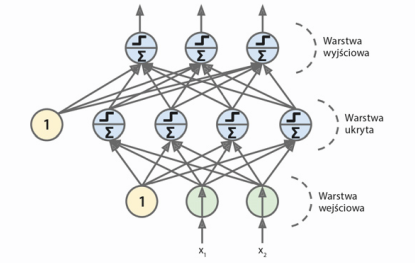
\includegraphics[scale=0.5]{gsn.png}
\caption{Perceptron wielowarstwowy z jedną warstwą ukrytą \cite{um}.}
\end{figure}

Zaproponowana w wzorze (3) metoda uczenia perceptronu nie zadziała w przypadku sieci
wielowarstwowej. Najpopularniejszą metodą uczenia sieci neuronowych 
jest \textbf{wsteczna propagacja}. Cały proces możemy przedstawić za pomocą kroków:

{\LinesNumbered
\begin{algorithm}[H]
 Wybór parametrów sieci (liczba warstw, liczba neuronów w warstwach itd.)\\
 Wagi inicjujemy losowo.\\
 Dla każdego neuronu wyjściowego obliczany jest błąd równy różnicy pomiędzy otrzymanym
 wynikiem $\hat{\vec{y}}$ a wartością oczekiwaną $\vec{y}$.\\
 Błędy propagowane są do poprzednich warstw.\\
 Modyfikacja wag na podstawie wartości błędu.\\
 Powtarzaj od \textbf{3} dla kolejnych wektorów uczących.\\
 Skończ algorytm jeśli przekroczymy ustaloną liczbę epok, lub średni błąd przestanie zauważalnie
 maleć.\\
 \caption{Procedura uczenia wielowarstwowej SSN.}
\end{algorithm}}
Średni błąd może być przestawiony przez wzór:
\begin{equation}
\label{wz:4}
	d = \frac{1}{2}(\vec{y} - \hat{\vec{y}})^2
\end{equation}
Podczas aktualizowania wag wybieramy te wartości dla których średni błąd jest najmniejszy, możemy
je znaleźć np. używając metodę gradientu prostego przy użyciu odwrotnego różniczkowania
automatycznego.
Propagację błędów do poprzednich warstw najlepiej pokazać na przykładzie:
\begin{figure}[H]
\centering
\includegraphics[scale=0.1]{back.png}
\caption{Schemat przykładowej SSN z jedną warstwą ukrytą oraz jednym nuronem w warswie
wyjściowej.}
\end{figure}
Dla powyższej sieci wagi łączące warstwę wejściową z ukrytą oznaczajmy przez 
$w_{ij}^{(1)}$, natomiast wagi łączące warstwę ukrytą z wyjściową przez 
$w_{ij}^{(2)}$. Zakładamy że powyższa sieć jako
funkcję aktywacyjna używa funkcji logistycznej $\sigma$ [\hyperref[sec:fa]{2.2.3}].
Wtedy postępujemy według kroków:\\
\begin{enumerate}
\item Obliczamy wartości neuronów  w warstwie ukrytej:
\begin{equation}
	h_i = \sum_{j} (w_{ij}^{(1)}x_j) + b_1
\end{equation}
\item Każdy neuron w warstwie ukrytej poddawany jest funkcji aktywacyjnej:
\begin{equation}
	\hat{h_i} = \sigma(h_i)
\end{equation}
\item W taki sam sposób obliczmy wartość na wyjściu:
\begin{align}
\begin{split}
	o' &= \sum_{i} (w_{i1}^{(2)}\hat{h_i}) + b_2\\
	\hat{o'} &= \sigma(o)
\end{split}
\end{align}
\item Kolejnym krokiem jest obliczenie błędu $d_o$ według wzoru (\hyperref[wz:4]{4}). 
\item Teraz rozpoczyna się etap propagacji wstecznej błędu, najpierw propagujemy błąd
do wag łączących warstwę ukrytą z warstwą wyjściową, wagi w sieci aktualizujemy przy pomocy wzoru:
\begin{equation}
\label{wz:8}
	w_{ij} = w_{ij} - \eta \pdv{d_o}{w_{ij}^{(2)}}
\end{equation}
Korzystając z reguły łańcuchowej wiemy że dla wag łączących warstwę ukrytą z warstwą wyjściową
powyższa pochodna przyjmuje postać:
\begin{equation}
	\pdv{d_o}{w_{ij}^{(2)}} = \pdv{d_o}{\hat{o'}} \pdv{\hat{o'}}{o'} \pdv{o'}{w_{ij}^{(2)}}
\end{equation}
Ponieważ wiemy, że powyższe pochodne są równe:
\begin{align}
\begin{split} 
	\pdv{d_o}{\hat{o'}} &= (\hat{o'} - o) \\
	\pdv{\hat{o'}}{o'} &=\hat{o'}(1 - \hat{o'}) \\
	\pdv{o'}{w_{ij}^{(2)}} &= \hat{h_i}
\end{split}
\end{align}
gdzie: $o$ - oczekiwana wartość na wyjściu.\\
Regułę modyfikacji wag podanych w wzorze (\hyperref[wz:8]{8}) możemy uprościć do postaci w której
wszystkie poprzednie wartości wcześniej policzyliśmy:
\begin{equation}
	w_{ij}^{(2)} = w_{ij}^{(2)} - \eta(\hat{o'} - o)\hat{o'}(1 - \hat{o'})\hat{h_i}
\end{equation}
\item Dla wag łączących warstwę wejściową z ukrytą pochodna $\pdv{d_o}{w_{ij}^{(1)}}$,
korzystając z reguły łańcuchowej otrzymujemy:
\begin{equation}
	\pdv{d_o}{w_{ij}^{(1)}} = \pdv{d_o}{\hat{o'}}\pdv{\hat{o'}}{o'}\pdv{o'}{\hat{h_j}}
	                          \pdv{\hat{h_j}}{h_j}\pdv{h_j}{w_{ij}^{(1)}}
\end{equation}
Pierwsze dwie pochodne policzyliśmy wcześniej pozostałe trzy są równe:
\begin{align}
\begin{split}
	\pdv{o'}{\hat{h_j}} &= w_{j1}^{(2)} \\
	\pdv{\hat{h_j}}{h_j} &= \hat{h_j}(1 - \hat{h_j})\\
	\pdv{h_j}{w_{ij}^{(1)}} &= x_i
\end{split}
\end{align}
Ostateczny wzór na modyfikację wag $w_{ij}^{(1)}$ jest więc równy:
\begin{equation}
	w_{ij}^{(1)} = w_{ij}^{(2)} - \eta (\hat{o'} - o)\hat{o'}(1 - \hat{o'})w_{j1}^{(2)}
	                                    \hat{h_j}(1 - \hat{h_j})x_i
\end{equation}
\end{enumerate}
Dla sieci z większą liczbą warstw ukrytych wzory modyfikacji wag dzięki regule łańcuchowej
rozrastałyby się o kolejne człony w sposób analogiczny jak w powyższym przykładzie.

\subsubsection{Funkcje aktywacyjne}
\label{sec:fa}
Aby powyższy algorytm przebiegał prawidłowo zamiast funkcji skokowej/signum wprowadzono inne 
funkcje aktywacji, ponieważ funkcje używane w przypadku pojedynczego perceptronu są złożone
jedynie z płaskich segmentów, co uniemożliwia korzystanie z gradientu. Poniżej znajdują się 
najczęściej używane \textbf{funkcje aktywacji} w SSN:
\begin{itemize}
\item \textbf{funkcja logistyczna}:\\
W każdym punkcie ma zdefiniowaną pochodną niezerową, dzięki czemu algorytm gradientu prostego
może na każdym etapie uzyskiwać lepsze wyniki. Jest ona używana w warstwie wyjściowej jeśli
zadaniem naszej sieci jest klasyfikacja obiektów na przynależność do dwóch rozłącznych klas.
Dodatkowo jest to funkcja używana przez neurony 
naturalne przez co uważana była za najlepszą funkcję aktywacyjną, lecz jak pokazała praktyka
w przypadku SSN inne funkcje sprawują się lepiej. Przyjmuje ona wartości z zakresu $(0,1)$.
\begin{equation}
\sigma(z) = \frac{1}{1 + e^{-z}}
\end{equation}
\item \textbf{funkcja tangensa hiperbolicznego}:\\
Jest S - kształtna, ciągła i różniczkowalna, podobnie jak funkcja logistyczna, 
ale zakres wartości wynosi $(-1, 1)$ a nie $(0, 1)$ jak w przypadku funkcji 
$\sigma$.
\begin{equation}
	\tanh(z) = \frac{e^z - e^{-z}}{e^z + e^{-z}}
\end{equation}
\item \textbf{funkcja ReLU}:\\
Jest ciągłą, ale nieróżniczkowalna dla $z = 0$. W praktyce jednak spisuje się znakomicie 
dodatkowo jest bardzo szybko obliczana. Aktualnie jest ona jak i jej odmiany najczęściej
używanymi funkcjami aktywacji dla warstw ukrytych i wejściowej. 
\begin{equation}
	ReLU(z) = \max(0, z)
\end{equation}
\item \textbf{funkcja softmax}:\\
Używana jest ona w warstwie wyjściowej jeśli nasza sieć ma obliczać
prawdopodobieństwa przynależności otrzymywanych obiektów  do klas 
(jest ich więcej niż 2 i wszystkie prawdopodobieństwa mają się sumować do $1$).
Model najpierw oblicza dla każdej klasy - $k$:
\begin{equation}
	s_k(\vec{x}) = \big(\vec{w}^{(k)}\big)^T\vec{x}
\end{equation}
gdzie: $\vec{w}^{(k)}$ - wyspecjalizowany wektor wag dla klasy $k$.\\
Po wyliczeniu $s_k(\vec{x})$ dla każdej klasy, obliczane jest odpowiednio znormalizowane 
prawdopodobieństwo przynależności danej próbki do klasy $k$:
\begin{equation}
	p_k = \frac{\exp\big(s_k(\vec{x})\big)}{\sum_{i=1}^{K} \exp\big(s_i(\vec{x})\big)}
\end{equation}
gdzie: $K$ - liczba klas.\\ 
Model prognozuje klasę o najwyższym prawdopodobieństwie:
\begin{equation}
	\hat{y} = \underset{k}{\text{argmax}}(p_k)
\end{equation}
Gdzie funkcja \textbf{argmax} zwraca indeks klasy dla której wartość $p_k$ jest największa.\\
\end{itemize}

\begin{figure}[H]
\centering
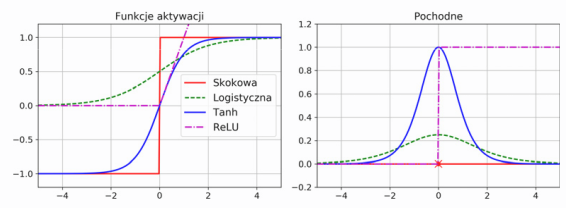
\includegraphics[scale=0.6]{f_a.png}
\caption{Funkcje aktywacyjne i ich pochodne. \cite{um}}
\end{figure}

\subsubsection{Inne rodzaje warstw SSN.}
W SSN oprócz \textbf{warstw gęstych} tzn.
gdzie każdy neuron w $i$-tej warstwie jest połączony z wszystkimi neuronami
znajdującymi się w warstwie nr. $i+1$,
używane są warstwy innego typu które pomagają sieciom
osiągać lepsze wyniki. Rodzaj warstwy też można rozważać jako kolejny
hiperparametr SSN. Oto kilka przykładowych warstw:
\begin{itemize}
\item \textbf{warstwa splotowa}:
Używane są one w zadaniach wizualnych. Neurony w pierwszej warstwie splotowej nie są
połączone z każdym pikselem obrazu wejściowego, lecz wyłącznie z pikselami
znajdującymi się w ich polu recepcyjnym.

\begin{figure}[H]
\centering
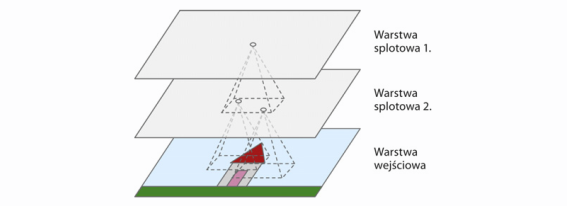
\includegraphics[scale=0.6]{cnn.png}
\caption{Warstwy CNN z prostokątnymi lokalnymi polami recepcyjnymi \cite{um}.}
\end{figure}

Dzięki powyższej strukturze sieć może koncentrować się na ogólnych cechach w pierwszej warstwie
ukrytej, następnie łączyć je w bardziej złożone kształty w kolejnych warstwach. Ogólnie neuron
znajdujący się w $i$-tym wierszu oraz $j$-tej kolumnie danej warstwy jest połączony z wyjściami 
neuronów poprzedniej warstwy zlokalizowanymi w rzędach od $i \cdot s_h$ do 
$i \cdot s_h + f_h-1$  i kolumnach
od $j \cdot s_w $ do $j \cdot s_w + f_w-1$
gdzie: $f_w/f_h$ - szerokość/wysokość pola recepcyjnego, $s_h, s_w$ definiują wartość 
\textbf{kroków} odpowiednio w kolumnach i rzędach. \textbf{Krok}  oznacza odległość
pomiędzy dwoma kolejnymi polami recepcyjnymi. Aby uzyskać takie same wymiary 
dla każdej warstwy najczęściej dodawane są zera wokół wejść. Krok i rozmiar pola recepcyjnego
musi podawać użytkownik tworzący warstwę więc są one kolejnymi hiperparametrami sieci.\\

Wagi neuronu mogą być przedstawione jako niewielki obraz o rozmiarze pola recepcyjnego, 
hiparapametr ten nazywamy \textbf{filtrem}.
Przykładowo filtrem może być macierz wypełniona zerami oprócz środkowej
kolumny zawierającej jedynki, neurony posiadające taki filtr będą ignorować wszystkie elementy
oprócz tych które znajdują się w środkowej linii.

\begin{figure}[H]
\centering
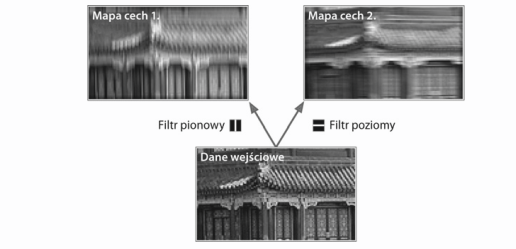
\includegraphics[scale=0.6]{filtr.png}
\caption{Dwie mapy cech otrzymane przy pomocy dwóch różnych filtrów \cite{um}.}
\end{figure}

Warstwa wypełniona neuronami o takim
samym filtrze nazywamy \textbf{mapą cech} która pomaga nam wyszczególnić elementy przypominające
użyty filtr. Warstwa splotowa składa się z kilku map cech o identycznych rozmiarach.
Każda mapa ma swoje wartości parametrów, dzięki czemu stosując różne filtry 
warstwa splotowa jest w stanie wykryć wiele cech w dowolnym obszarze obrazu.
Dodatkowo obrazy wejściowe składają się również z kilu warstw, po jednej na każdy kanał
barw. Zazwyczaj są to trzy kanały - czerwony, zielony i niebieski lub jeden dla obrazów
czarno-białych.


\begin{figure}[H]
\centering
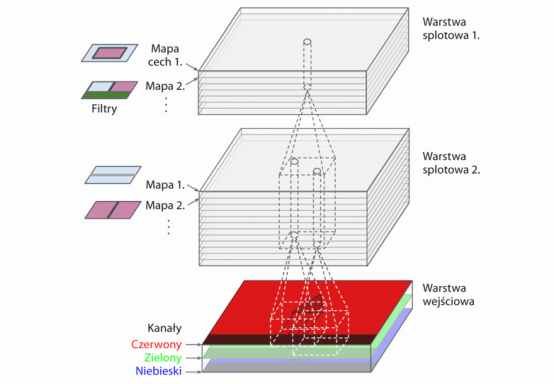
\includegraphics[scale=0.6]{rgb_cnn.png}
\caption{Warstwa splotowa zawierająca wiele cech, oraz zdjęcie z trzema kanałami barw \cite{um}.}
\end{figure}

\item \textbf{warstwa łącząca}:
Jej celem jest zmniejszenie obrazu wejściowego w celu zredukowania obciążenia obliczeniowego,
wykorzystania pamięci i liczby parametrów. Tak samo jak w warstwach splotowych neurony 
łączą się z wyjściami określonej liczby neuronów poprzedniej warstwy, które mieszczą się w
obszarze pola recepcyjnego. Jednakże warstwa ta nie zawiera wag, jej zadaniem jest gromadzenie
danych przy pomocy funkcji agregacyjnej np. maksymalizującej lub uśredniającej.

\begin{figure}[H]
\centering
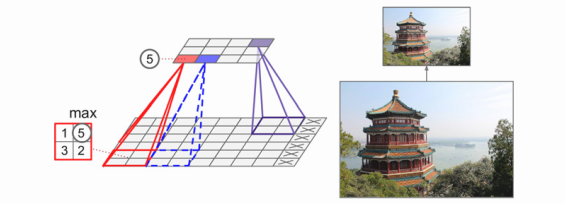
\includegraphics[scale=0.6]{pool.png}
\caption{Maksymalizująca warstwa łącząca, gdzie rozmiar jądra łączącego to 2x2 \cite{um}.}
\end{figure}

\item \textbf{warstwa porzucania}:\\
Warstwa ta dla poprzedniej warstwy aplikuję technikę \textbf{porzucania} tzn. że
każdy neuron znajdujący się w tej warstwie w poszczególnym przebiegu może zostać całkowicie
pominięty w procesie uczenia. Szansa na porzucenie jest hiperparametrem i nazywana jest 
\textbf{współczynnikiem porzucenia}.

\begin{figure}[H]
\centering
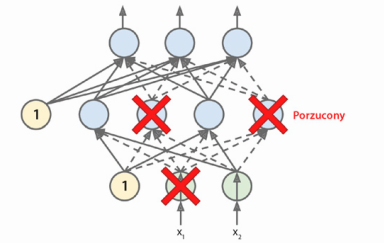
\includegraphics[scale=0.6]{dropout.png}
\caption{Przykład porzucania \cite{um}.}
\end{figure}

\end{itemize}
Istnieje wiele innych rodzajów warstw w SSN (np. rekurencyjne) lecz opisałem tyko warstwy
użyte w moim programie. Z tego samego powodu jedyną opisaną przeze mnie architekturą jest
\textbf{jednokierunkowa sieć neuronowa}(sygnał biegnie w jednym kierunku).

\section{Mikro - GA dla SSN}
\subsection{Modyfikacja AG}
SSN posiadają dużą liczbę hiperparametrów i wpływ każdego z nich na efektywność sieci jest
zależny od wykonywanego zadania, więc jeżeli wybieramy je ręcznie musimy to robić
metodą prób i błędów.
Aby zautomatyzować ten proces wykorzystam w tym celu Algorytm Genetyczny, który porównując
sieci z różnymi wartościami hiperparametrów wybierze możliwie najlepszą według zadanej 
metryki. Z powody dużej ilości hiperparamtetrów w SSN musiałem wybrać ich ograniczoną ilość
(wybrane hiperparametry opisane są w podrozdziale [\hyperref[sec:ssn]{2.2}]).
Modyfikując AG musimy pamiętać, że będziemy operować na sieciach o różnych rozmiarach, lecz
użytkownik musi wybrać ich maksymalną liczbę. Musi on też wybrać typ wykonywanego zadania 
(klasyfikacja lub regresja), ponieważ do każdego typu przypisywana jest inna metryka
oceny jakości sieci (patrz [\hyperref[sec:ocena]{3.4}]).
Implementując operację krzyżowania i mutacji potrzebne jest uwzględnienie aby tworzyły one
prawidłowe sieci (wymagana kolejność warstw, liczba warstw nieprzekraczająca maksymalnej
 patrz [\hyperref[sec:ossn]{3.2}]).


Aby użyć AG to tego zadania musimy zmodyfikować jego tradycyjną odmianę.
Poniżej znajduje się lista wszystkich 
parametrów zmodyfikowanego algorytmu oraz użyte dla nich oznaczenia
ich rola natomiast zostanie omówiona w kolejnych podrozdziałach.
\begin{table}[H]
\centering
\begin{tabular}{|c|c|}
	\hline
	Nazwa parametru & Oznaczenie \\
	\hline
	Współczynnik sprawdzianu krzyżowego & $\gamma_v$ \\
	Prawdopodobieństwo mutacji & $\rho_m$ \\
	Prawdopodobieństwo dodania warstwy & $\gamma_l$ \\
	Maksymalna liczba warstw & $\mathcal{A}$ \\
	Współczynnik skalowania rozmiaru sieci (patrz \hyperref[sec:ocena]{3.3}) & $\alpha$ \\
	Rozmiar populacji & $n$ \\
	Rozmiar turnieju & $n_t$ \\
	Dopuszczalne podobne modele & $\gamma_c$\\
	Liczba epok treningowych & $\gamma_t$\\
	Liczba generacji & $\gamma_g$\\
	Liczba eksperymentów & $\gamma_r$\\
	\hline
\end{tabular}
\caption{\label{tab:params}Parametry AG dla SNN.}
\end{table}

Ponieważ zależy nam na szybkości wykonywanych obliczeń zastosowana została odmiana 
\textbf{micro-GA} gdzie liczba dozwolonych generacji jest niewielka. Dodatkowo aby przyśpieszyć
działanie algorytmu SSN są trenowane przez ograniczoną liczbę epok tzw. \textbf{uczenie
częściowe}.

\begin{algorithm}[H]
 \SetAlgoLined
 \KwData{Treningowy i walidacyjny zbiór danych $\mathcal{D}_t$, $\mathcal{D}_v$}
 \KwIn{Parametry algorytmu.}
 \KwOut{Najlepiej przystosowana SSN $\phi^{*}$}
 \caption{Zmodyfikowany Algorytm Genetyczny wybierający hiperparametry SSN.}
 Niech $t_e = 0$ będzie licznikiem wykonanych przebiegów AG.\\
 Niech $\mathcal{S}$ zbiór najlepszych rozwiązań.\\
 \While{$t_e < \gamma_r$}{
 	Niech $t = 0$ będzie licznikiem generacji.\\
	Stwórz i losowo zainicjalizuj początkową populację $\mathcal{C}(0)$, zawierającą 
	$n$ osobników, gdzie $n \leq 10$.\\
	\While{$t<\gamma_g \lor$ warunek wczesnego ko\'nca dla $\mathcal{C}(t)$ nie 
	       jest spełniony}{
		Oblicz funkcję przystosowania $c(\phi)$ dla każdego osobnika w populacji.\\
		Wykonaj selekcję tworząc populację potomstwa $\mathcal{O}(t)$.\\
		Wykonaj operację krzyżowania i mutacji na osobnikach z $\mathcal{O}(t)$.\\
		$\mathcal{C}(t + 1) = \mathcal{O}(t)$.\\
		$t = t + 1$.\\
	}
	Do $\mathcal{S}$ dodaj najlepszego osobnika z poprzedniego przebiegu.\\
	$t_e = t_e + 1$.\\
  }
  Znormalizuj koszt dla każdego modelu w $\mathcal{S}$.\\
  Najlepszym modelem jest osobnik z $\mathcal{S}$ dla którego funkcja przystosowania
  przyjmuję najniższą wartość.
\end{algorithm}

\subsection{Reprezentacja SSN w AG}
\label{sec:ossn}
Z powodu złożoności SSN musiałem zrezygnować ze standardowej reprezentacji osobników 
jako ciągi binarne. Użytym przeze mnie modelem jest kodowanie oparte na liście tablic tzn.
każda warstwa sieci jest reprezentowana jako tablica w której każde pole ma z góry określone 
znaczenie. W tej reprezentacji warstwy przyjmują postać:\\
\begin{figure}[H]
\centering
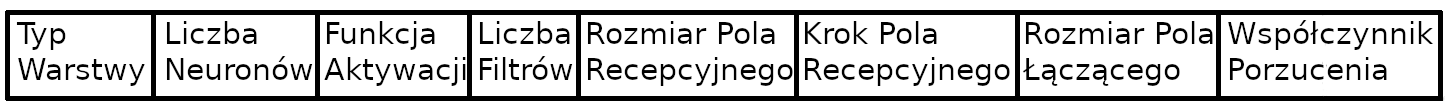
\includegraphics[scale=0.30]{dnn_genome.png}
\caption{Schemat reprezentacji warstw w genotypie reprezentującym SSN.}
\end{figure}
Dla poszczególnych typów sieci używane są inne pola:\\
\begin{table}[H]
\centering
\begin{tabular}{|c|c|c|}
	\hline
	Nr. & Rodzaje SSN & Rodzaje Warstw\\
	\hline
	1 & Perceptron wielowarstwowy/Sieć splotowa & Wszystkie warstwy\\
	2 & Perceptron wielowarstwowy & Gęsta\\
	3 & Perceptron wielowarstwowy/Sieć splotowa & Gęsta i Splotowa \\
	4 & Sieć splotowa & Splotowa\\
	5 & Sieć splotowa & Splotowa\\
	6 & Sieć splotowa & Splotowa\\
	7 & Sieć splotowa & Łącząca\\
	8 & Perceptron wielowarstwowy/Sieć splotowa & Porzucania\\
	\hline
\end{tabular}
\caption{\label{tab:zakres}Hiperparametry SSN używane przez poszczególne rodzaje sieci i 
         warstwy.}
\end{table}

Osobniki więc będą listą takich tablic.
Warstwa wejściowa i wyjściowa jest ustalona 
przez zadanie jakie ma wykonywać sieć np. jeśli trenowana sieć ma rozpoznawać ręcznie pisane
cyfry wiemy że w warstwie  wyjściowej musi pojawić się 10 neuronów z funkcją aktywacyjną
typu softmax.
Generując jednak pozostałe warstwy musimy pamiętać że warstwy nie mogą być ułożone losowo
(np. nie mogą występować dwie warstwy porzucania po sobie). Poniżej znajdują się odpowiednie
mapowania typów warstw i użytych funkcji aktywacji na liczby całkowite oraz odpowiednie zasady 
łączenia warstw w generowanych osobnikach.\\

\begin{table}[H]
\centering
\begin{tabular}{|c|c|c|}
	\hline
	Typ warstwy & Nazwa & Dozwoleni następcy \\
	\hline
	1 & Warstwa Gęsta & 1, 4\\
	2 & Splotowa & 1, 2, 3, 4\\
	3 & Łącząca & 1, 2\\
	4 & Porzucenia & 1, 2 \\
	\hline
\end{tabular}
\caption{\label{tab:rules}Mapowanie typów warstw oraz zasady łączenia warstw.}
\end{table}
\begin{table}[H]
\centering
\begin{tabular}{|c|c|}
	\hline
	Typ funkcji & Nazwa\\
	\hline
	1 & Sigmoid \\
	2 & Tangens hiperboliczny \\
	3 & ReLU \\
	4 & Softmax \\
	5 & Liniowa \\
	\hline
\end{tabular}
\caption{\label{tab:fun}Mapowanie funkcji aktywacyjnych.}
\end{table}
Rodzaje filtrów są generowane przez bibliotekę \texttt{tensorflow} w której implementuję 
powyższy algorytm (patrz rozdział [\hyperref[sec:imp]{4}]).
Reszta hiperparametrów należy do całkowitych/rzeczywistych z pewnego zadanego przedziału 
wyspecjalizowanego do danych dla których szukamy optymalnej sieci
[\hyperref[tab:fm_zakes]{Tab. 9}].\\
Dodanie innych typów warstw (np. rekurencyjnych) i funkcji nie powinno być problemem, jedynie
trzeba pamiętać o dodaniu odpowiednich zasad budowania dla nich.
Przykładowy genotypem reprezentującym SSN jest:\\
\begin{align*}
	  G = \big[[1, 784, 3, 0, 0, 0, 0, 0], [4, 0, 0, 0, 0, 0, 0, 0.54],\\
	          [1, 300, 3, 0, 0, 0, 0, 0], [4, 0, 0, 0, 0, 0, 0, 0.28],\\ 
	          [1, 100, 3, 0, 0, 0, 0, 0], [1, 10, 4, 0, 0, 0, 0, 0]\big]
\end{align*}
Dekodując powyższy genotyp otrzymujemy sieć złożoną z następujących warstw:\\
\begin{table}[H]
\centering
\begin{tabular}{|c|c|c|c|}
	\hline
	Typ warstwy & Liczba Neuronów & Funkcja Aktywacji & Wsp. Porzucenia \\
	\hline
	Gęsta & 784 & ReLU & N/A \\
	Porzucanie & N/A & N/A & 0.54\\
	Gęsta & 300 & ReLU & N/A \\
	Porzucanie & N/A & N/A & 0.28\\
	Gęsta & 100 & ReLU & N/A \\
	Gęsta & 10 & Softmax & N/A \\
	\hline
\end{tabular}
\caption{\label{tab:gen1}Genotyp $G$ przedstawiony w postaci tabeli.}
\end{table}


\subsection{Generowanie w populacji początkowej}
Generując genotypy w populacji warstwa pierwsza wyznacza typ SSN(np. jeśli pierwszą warstwą
jest warstwa gęsta to sieć będzie perceptronem wielowarstwowym, a jeśli pierwszą warstwą
będzie warstwa splotowa sieć będzie siecią splotową).
Warstwa wejściowa i wyjściowa dla każdego osobnika jest taka sama ponieważ
są one zależne od danych na jakich trenujemy oraz od zadania jakie ma nasza sieć wykonywać
(klasyfikacja lub regresja), dlatego w populacji początkowej musimy losowo generować tylko
warstwy ukryte.
Proces generowania możemy opisać przy pomocy pseudokodu:\\
\newline
\begin{algorithm}[H]
	\KwOut{Zainicjalizowana populacja początkowa $\mathcal{C}(0)$.}
	Niech $\mathcal{C}(0)$ oznacza populację początkową wielości
	$n$, gdzie genotypy tej populacji możemy oznaczyć przez $\vec{x}_i$.\\
	\For{Dla każdego i, gdzie $1 \leq i \leq$ $n$} {
		Dla wszystkich warstw poza wyjściową (która ma z góry określoną 
		funkcję aktywacji) losujemy funkcję aktywacji $f$.\\
		\While{Liczba warstw $\vec{x_i} \leq \mathcal{A}$
		        \hyperref[tab:params]{[Tab 2]}} {
			Wylosuj typ warstwy a następnie wartości używanych przez nią 
			parametrów.\\
			Wylosuj liczbę $U$ przy pomocy płaskiego rozkładu prawdopodobieństwa
			z przedziału $[0, 1]$.\\
			Oblicz $\rho_l = 1 - \sqrt{1 - U}$.\\
			\If{$\rho_l < \gamma_l$\hyperref[tab:params]{[Tab 2]}}{
				Jeśli wygenerowana warstwa jest kompatybilna z warstwą
				poprzednią dodaj ją do genotypu.\\
			}
			\Else{
				Kończymy dodawanie warstw dla $\vec{x}_i$.\\
			}
		}
	}
	\caption{Generowanie populacji początkowej.}
\end{algorithm}

\subsection{Funkcja oceny dla SSN}
\label{sec:ocena}
Celem algorytmu jest znalezienie sieci $\phi^{*}$ osiągającej jak najlepszy wynik jednocześnie
ograniczając liczbę trenowalnych parametrów, więc jest to problem optymalizacyjny 
przedstawiony za pomocą wzoru:
\begin{equation}
	\underset{\phi}{\min}\big(p(\phi), w(\phi)\big)
\end{equation}
gdzie:\\
$p(\phi)$ - miara jakości sieci(np. błąd predykcji dla klasyfikacji, błąd średniokwadratowy 
\textbf{MSE} dla regresji),\\
$w(\phi)$ - liczba trenowalnych parametrów zwana \textbf{rozmiarem sieci}.\\
Jeżeli jednak chcielibyśmy znaleźć bezpośrednio rozwiązanie powyższego równania
prowadziłoby to do zadania optymalizacji wielokryterialnej. Aby uprościć to zadanie
definiujemy funkcję oceny, względem której osobniki w populacji będą porównywane:
\begin{equation}
	c(\phi) = (1 - \alpha)p(\phi) + \alpha w(\phi)
\end{equation}

Jednak powinniśmy jeszcze przeskalować $p(\phi)$ i $w(\phi)$ aby ich wartości były podobnego 
rzędu. Niech $\vec{p} = \{p(\phi_1), ..., p(\phi_n)\}$ będzie wektorem ocen aktualnej populacji,
wtedy po znormalizowaniu $\vec{p}^{*} = \frac{\vec{p}}{||\vec{p}||}$ zakres wartości ocen sieci
będzie z przedziału $p^{*}(\phi_i) \in [0, 1]$ dla każdego $i$. Niech $\mathcal{A}$ oznacza
maksymalną liczbę warstw w sieci, oraz $\mathcal{N}$ oznacza maksymalną liczbę neuronów w 
warstwie wtedy maksymalna wartość rozmiaru sieci jest równa $w(\phi) = \mathcal{N}^2\mathcal{A}$.
Ponieważ chcemy aby sieci o podobnych rozmiarach miały podobną wartość $w(\phi)$,
ostatnie trzy cyfry rozmiaru zamieniamy na zera otrzymując $w'(\phi)$.
Następnie aby skalami zbliżyć się do 
wartości ocen  wyznaczamy $w^{*}(\phi) = \log_{10}w'(\phi)$ (rozmiaru sieci
nie normalizujemy podobnie jak wartości ocen ponieważ chcemy aby różnica w rozmiarze
miała większe wpływ na różnice w funkcji ocen), co nam daje wartości
rzędu $\log_{10}(\mathcal{N}^2\mathcal{A})$.\\
Wtedy odpowiednio przeskalowana funkcja oceny wyrażona jest wzorem:
\begin{equation}
	c(\phi) = \log_{10}(\mathcal{N}^2\mathcal{A})(1 - \alpha)p^{*}(\phi) + \alpha w^{*}(\phi)
\end{equation}

\subsection{Selekcja}
Aby wygenerować $n$ potomków potrzebujemy $2n$ rodziców wybranych z bieżącej populacji.
Do tego celu wykorzystamy odmianę \textbf{binarnej selekcji turniejowej}:\\
\begin{algorithm}[H]
 \KwIn{Aktualna generacja $\mathcal{C}(t)$.}
 \KwOut{Pula rodzicielka następnej generacji}
 Niech $\mathcal{P}$ - zbiór rodziców.\\
 Wybierz losowo $m$ rodziców gdzie $m < n$.\\
 \While{nie wybrano 2n rodziców} {
	Porównaj parami wybrane genotypy , lepiej przystosowany dodaj do $\mathcal{P}$.
	Pary tworzymy przez branie kolejnych dwójek z puli rodziców (np. pierwszy osobnik z 
	drugim itd.).
 }
 \caption{Binarna selekcja turniejowa dla SSN.}
\end{algorithm}
W powyższej procedurze im większa wartość $m$ tym większe jest prawdopodobieństwo wybrania
najlepszych osobników jako rodzica.

\subsection{Krzyżowanie}
Ponieważ standardowe operatory genetyczne nie będą działać dla zmodyfikowanego kodowania
genotypów, je również trzeba zmodyfikować. Wybranym krzyżowaniem jest zmodyfikowane krzyżowanie
dwupunktowe. Wykonując krzyżowanie musimy pamiętać, że nie każda warstwa może występować po 
każdej innej. Przykładowa dla dwóch rodziców $G_1$, $G_2$ po wybraniu punktów $(r_1, r_2)$ z 
$G_1$ i $(r_3, r_4)$ z $G_2$ (gdzie $r_i$ oznacza indeks warstwy), może się stać że warstwa
$r_3$ nie może być zamieniona z warstwą $r_1$ lub $r_4$ z $r_2$ z powodu niekompatybilności
z warstwą poprzednią [\hyperref[tab:rules]{Tab4}].\\
\begin{algorithm}[H]
	\KwIn{Dwa genotypy $G_1$, $G_2$.}
	\KwOut{Nowy potomek $G_3$.}
	Losowo wybierz dwa punkty z $G_1$ gdzie $r_1 \leq r_2$.\\
	\If{$r_1$ = $r_2$} {
		$r_2$ = \text{len}($G_1$) - 1
	}
	Znajdź wszystkie pary punktów $(r_3, r_4)_i$ w $S_2$ kompatybilne z $(r_1, r_2)$,
	gdzie $r_3 < r_4$ i $len(G_1) + (r_4 - r_3) - (r_2 - r_1) < \mathcal{A}$
	(sprawdzamy czy nie przekraczamy maksymalnej liczby warstw).\\
	Losowo wybierz jedną z par $(r_3, r_4)_i$.\\
	W $G_1$ usuń warstwy z przedziału $[r_1, r_2]$ a następnie wstaw tam
	warstwy z przedziału $[r_3, r_4]$ wzięte z $G_2$. Nowy genotyp oznacz jako $S_3$.\\
	W $G_3$ zmień w warstwach wziętych z $G_2$ funkcję aktywacji, na funkcję 
	używaną w warstwach wziętych z  $G_1$.
	\caption{Krzyżowanie dwupunktowe dla SSN.}
\end{algorithm}
Operacja ta dla dwóch poniższych genotypów będzie przebiegać następująco \cite{ams}:\\
\begin{align*}
	G_1 = \big[[1, 784, 2, 0, 0, 0, 0, 0], [4, 0, 0, 0, 0, 0, 0, 0.54],\\ 
	            [1, 300, 2, 0, 0, 0, 0, 0], [4, 0, 0, 0, 0, 0, 0, 0.28],\\
		    [1, 100, 2, 0, 0, 0, 0, 0], [1, 10, 4, 0, 0, 0, 0, 0]\big]
\end{align*}
\begin{align*}
	G_2 = \big[[1, 64, 1, 0, 0, 0, 0, 0], [4, 0, 0, 0, 0, 0, 0, 0.22],\\
		    [1, 333, 1, 0, 0, 0, 0, 0], [1, 420, 1, 0, 0, 0, 0, 0],\\
		    [1, 77, 1, 0, 0, 0, 0, 0], [4, 0, 0, 0, 0, 0, 0, 0.44],\\
		    [1, 10, 4, 0, 0, 0, 0, 0]\big]
\end{align*}
Dla $r_1 = 1$ i $r_2 = 3$ zbiór wszystkich możliwych par $(r_3, r_4)_i$ dla $G_1$ i $G_2$ wynosi:
\begin{equation*}
	[(0,2),(0,4),(0,5),(1,2),(1,4),(1,5),(2,4),(2,5),(4,5)]
\end{equation*}
Zakładając że wylosowaliśmy punkty $(2,4)$ potomek $G_3$ po wykonanej operacji krzyżowania
jest równy:
\begin{align*}
	G_3 = \big[[1, 784, 2, 0, 0, 0, 0, 0], [1, 333, 2, 0, 0, 0, 0, 0],\\
	            [1, 420, 2, 0, 0, 0, 0, 0], [1, 77, 2, 0, 0, 0, 0, 0],\\ 
		    [1, 100, 3, 0, 0, 0, 0, 0], [1, 10, 4, 0, 0, 0, 0, 0]\big]
\end{align*}
Jak widzimy funkcje aktywacji w warstwach pobranych z $G_2$ zostały zamienione na funkcję
używaną w $G_1$.\\

\subsection{Mutacja}
Mimo że mutacja nie jest potrzebna w mikro-AG, została ona dodana aby jeszcze bardziej
zróżnicować modele i potencjalnie zwiększyć szanse na otrzymanie lepszych rozwiązań.
Zmodyfikowana operacja mutacji jest bardzo podobna do swojej klasycznej wersji.
Każdy model z populacji potomków może podlec mutacji przy prawdopodobieństwie $\rho_m$, wtedy:
\begin{itemize}
	\item Losowo wybierz jedną z warstw, a następnie zmień jeden z jej używanych parametrów
		zgodnie z tabelą [\hyperref[tab:zakres]{Tab 3}].
	\item Zmień funkcję aktywacji, a następnie skoryguj ją w pozostałych warstwach 
	oprócz ostatniej.
	\item Dodaj warstwę porzucenia jeśli może ona występować po zmienianej warstwie 
	      [\hyperref[tab:rules]{Tab 4}].
\end{itemize}

\subsection{Warunek końca}
W Algorytmie Genetycznym może dojść do sytuacji w której zmiany w kolejnych pokoleniach są
niezauważalne, wtedy bez konsekwencji można zakończyć aktualny przebieg algorytmu. Możemy to
zaimplementować definiując odpowiedni warunek końca. Warunek ten można oprzeć na funkcji oceny
wiemy jednak że sieci o podobnej strukturze będą miały zbliżone wartości dla tej funkcji.
Dlatego warunek końca możemy oprzeć definiując \textbf{odległość} między genotypami mówiąca nam
jak zbliżone są do siebie dwie SSN.\\
Niech $G^{(i)}$ - oznacza $i$-tą warstwę sieci $S$. Wtedy przy założeniu 
len$(G_2) \geq$ len$(G_1)$
odległość $d(G_1, G_2)$ miedzy dwoma genotypy reprezentującymi SSN możemy obliczyć według 
algorytmu:

\begin{algorithm}[H]
	\KwIn{Dwa genotpy $G_1$, $G_2$.}
	\KwOut{Odległość między $G_1$ a $G_2$.}
	Niech $d = 0$ - odległość między $G_1$ a $G_2$.\\
	\For{Dla każdego i, gdzie $1 \leq i \leq$ len$(G_1)$} {
		$d = d + ||G_2^{(i)} - G_1^{(i)}||$.\\
	}
	\For{Dla każdego i, gdzie len$(G_1) < i \leq$ len$(G_2)$} {
		$d = d + ||G_2^{(i)}||$.\\
	}
	\caption{Odległość między dwoma SSN.}
\end{algorithm}

Dla powyższej definicji $d$ jeśli $G_1 = G_2$ to $d(G_1, G_2) = 0$, wiec pozwala nam ona określić
stopień podobieństwa dwóch osobników.\\
Aktualny przebieg AG kończymy więc gdy co najmniej $\gamma_c$ par spełnia 
$d(S_1, S_2) \leq \varepsilon$.\\
Gdzie: $\varepsilon$ to pewna zadana dokładność, a $\gamma_c$ jest parametrem AG.


\section{Implementacja}
\label{sec:imp}
Do zrealizowania opisanego wyżej AG użyłem języka \texttt{python} wraz z biblioteką 
implementującą wiele operacji numerycznych \texttt{numpy}, natomiast do budowania i trenowania
sieci neuronowych wykorzystałem popularną bibliotekę \texttt{tensorflow}. Aby przyśpieszyć
trenowanie sieci wykorzystałem platformę \texttt{Google Colab}, gdzie korzystając z popularnej
formy \texttt{jupyter notebooków} mamy darmowy dostęp przez chmurę do karty graficznej
przyśpieszającej trenowanie SSN, co znacznie skraca czas wykonania naczego algorytmu.
Algorytm podzieliłem na cztery programy z których każdy wykonuję jedną z funkcji:
\begin{itemize}
\item Przechowywanie zasad budowania SSN oraz parametrów potrzebnych do wykonania algorytmu.
\item Dla danego genotypu budowanie sieci przy pomocy biblioteki \texttt{tensorflow}, oraz
zwrócenie oceny oraz wielkości sieci.
\item Implementacja klasy reprezentującej pojedynczy genotyp, która ułatwia implementacje
operacji związanych z AG.
\item Implementacja klasy reprezentującej AG gdzie znajdują się funkcję wykonujące algorytmy
opisane w pseudokodach w rozdziale trzecim.
\end{itemize}
Programy opisane są w poniższych podrozdziałach:\\

\subsection{Reguły budowania SSN.}
Pomocniczy plik \texttt{building\_rules.py} zawiera typy wyliczeniowe takie jak np.
\texttt{LayerType} zwiększające czytelność kodu, oraz słowniki które:
\begin{itemize}
\item opisują maksymalne wartości opisane w tabeli [\hyperref[tab:zakres]{Tab 3}].
\item zawierają reguły budowania sieci podane w tabeli [\hyperref[tab:rules]{Tab 4}].
\item opisują funkcje aktywacyjne dostępne dla warstwy danego typu.
\end{itemize}

\subsection{Budowanie SSN zgodnej z genotypem.}
Program \texttt{building\_models.py} zawiera funkcje które dla każdego genotypu budują sieci neuronowe 
przy pomocy biblioteki \texttt{tensorflow}, która od aktualizacji \texttt{2.0}
umożliwia proste budowanie modeli przy pomocy modułu \texttt{keras}. Poszczególne 
rodzaje warstw mają swoje gotowe implementacje oraz reguły zaimplementowane w wyżej opisanym
programie dają nam gwarancję że modele te będą poprawne. Algorytm genetyczny posiada wszystkie
potrzebne parametry do przeprowadzenia procesu trenowania i zwrócenia potrzebnych dla niego
wartości tzn. oceny wydajności sieci oraz liczby trenowalnych parametrów. Musimy pamiętać
aby dla zadań regresji i klasyfikacji użyte zostały odpowiednie metryki jakości SSN.
W mojej implementacji wykorzystałem poniższe metryki:\\
\begin{table}[H]
\centering
\begin{tabular}{|c|c|}
	\hline 
	Rodzaj problemu & Metryka \\
	\hline
	Klasyfikacja & Precyzja \\
	Regresja & Błąd Średniokwadratowy\\
	\hline
\end{tabular}
\caption{\label{tam:met}Użyte metryki.}
\end{table}

\subsection{Reprezentacja genotypu}
W \texttt{nn\_genome.py} znajduję się klasa opakowująca genotypom przy pomocy listy list.
Język \texttt{python} posiada implementacje listy która idealnie nadaję się do AG dla SSN, 
ponieważ może ona zawierać wartości różnego typu więc może ona np. posiadać jednocześnie
pole opisujące liczbę neuronów w warstwie, która jest typu całkowitoliczbowego (\texttt{int}),
oraz pole opisujące współczynnik porzucenia co jest typu zmiennoprzecinkowego 
(\texttt{float}).

\subsection{Algorytm Genetyczny}
Głownym plikiem jest \texttt{nn\_optimizer.py} w którym znajduję się największa liczba operacji,
ponieważ przy pomocy klasy \texttt{NNOptimizer} implementujemy cały przebieg AG.
Projektując interfejs tej klasy inspirowałem się biblioteką implementującą
algorytmy uczenia maszynowego \texttt{scikit-learn}. Proces poszukiwania
optymalnej sieci neuronowej z poziomu użytkownika jest bardzo prosty, jedyne co musi zrobić
to stworzyć instancję podanej wyżej klasy do której konstruktora musimy podać typ wykonywanego
zadania (klasyfikacja lub regresja) oraz ewentualnie parametry opisane w tabeli 
[\hyperref[tab:params]{Tab 2}]. Nie jest to jednak obowiązkowe ponieważ posiada ona dla nich
wartości domyślne.
Następnie cały algorytm genetyczny oraz finalne wytrenowanie otrzymanej sieci z pełną
liczbą epok odbywa się przez wywołanie metody \texttt{fit} która pobiera jako argumenty
dane oraz oczekiwane wartości. Poniżej przykładowe wywołanie programu:\\
\begin{center}
	\texttt{nn\_optimizer.NNOptimizer.fit(X, y)}\\
\end{center}
gdzie \texttt{X, y} - zbiór danych podzielony na dane wejściowe i oczekiwane wartości.\\
Interfejs ten umożliwia rozwiązanie jakiegoś problemu z użyciem uczenia maszynowego
nawet jeśli użytkownik nie posiada wiedzy na temat przebiegu algorytmu który dana klasa 
implementuje.\\
\newline
Aby przyśpieszyć wykonywanie AG możemy w każdej generacji budować i trenować 
modele przy pomocy programu \texttt{building\_models.py} równolegle. Jednak trenowanie tylu
sieci jednocześnie jest procesem potrzebujących wiele zasobów, więc można tę opcję wyłączyć
podając wartość argumentu funkcji \texttt{train\_parallel=False} wywołując funkcję 
\texttt{fit}.
Równoległość zaimplementowałem przy pomocy wbudowanej biblioteki \texttt{python'a}
\texttt{multiprocessig} i jej klasy \texttt{Pool}, która posiada
funkcję \texttt{pool} do której jako argumenty mogę podać funkcję budującą i trenującą 
SSN oraz populację genotypów, wtedy dla każdego osobnika zostanie utworzony osobny proces
i możliwe będzie równoległa ewaluacja osobników.


\section{Otrzymane wyniki}
Działanie algorytmu przetestowałem zarówno dla problemu kwalifikacji jak i  regresji
Użyłem do tego dwa zbiory danych \textbf{Fashion Mnist} i \textbf{Boston housing}. 
Zbiory te są stosunkowo małe (fashion mnist zawiera 70 tyś zdjęć), aby mógł algorytm 
mógł przetestować dla różnych wartości parametrów AG dla SSN.
\subsection{Fashion MNIST}
Jest to zbiór artykułów z sklepu Zalando. Każdy obraz jest rozmiaru 28x28 pikseli w odcieniach 
szarości:

\begin{figure}[H]
\centering
\includegraphics[scale=0.8]{fashin_mnist.png}
\caption{Przykładowe obrazki z Fashion Mnist.}
\end{figure}
Każdy obrazek ma przypisaną jedną z 10 klas zmapowanych od liczb całkowitych od 1-9.
\begin{table}[H]
\centering
\begin{tabular}{|c|c|}
	\hline
	Nr. & Klasa \\
	\hline
	0 & T-shirt/top \\
	1 & Trouser \\
	2 & Pullover \\
	3 & Dress \\
	4 & Coat \\
	5 & Sandal \\
	6 & Shirt \\
	7 & Sneaker \\
	8 & Bag \\
	9 & Ankle boot \\
	\hline
\end{tabular}
\caption{\label{tab:fmcls}Klasy zbioru Fashion Mnist.}
\end{table}
Więc jest to zadanie klasyfikacji gdzie gdzie nasza sieć próbuje podanemu zdjęciu przypisać jedną
z 10 klas.\\
Algorytm był testowany kilkukrotnie na tym zbiorze zmieniając wartości $\alpha$, lecz reszta
parametrów AG była stała [\hyperref[tab:params]{Tab 2}]\\
\begin{table}[H]
\centering
\begin{tabular}{|c|c|}
	\hline
	Parametr & Wartość\\
	\hline
	 $\gamma_v$ &0.4\\
	 $\rho_m$ &0.1\\
	 $\gamma_l$& 0.5\\
	 $\mathcal{A}$ &10\\
	 $n$  &10\\
	 $n_t$  &4\\
	 $\gamma_c$  &3\\
	 $\gamma_t$ &10\\
	 $\gamma_g$ &10\\
	 $\gamma_r$ &5\\
	\hline
\end{tabular}
\caption{\label{tab:fm_params}Parametry AG dla Fashion Mnist.}
\end{table}
Ograniczone maksymalnymi wartościami zostały również optymalizowane hiperparametry sieci 
[\hyperref[tab:zakres]{Tab 3}], aby podczas generowania początkowej populacji 
nie zostały stworzone sieci o za dużej wielkości. Zapobiega to również zjawiskowi 
\textbf{przetrenowania} tzn. z powodu dużej złożoności sieć dopasowuję się on niemal idealnie
do danych na których przeprowadza proces uczenia, przez co sieć na danych spoza puli treningowej
nie potrafi poprawnie przewidzieć oczekiwanych wartości.

\begin{table}[H]
\centering
\begin{tabular}{|c|c|}
	\hline
	Nazwa & Zakres Wartości  \\
	\hline
	Liczba neuronów           & $8*x$ dla $x\in \{1, ...,32\}$\\
	Liczba Filtrów            & $8*x$ dla $x\in \{1, ...,16\}$\\
	Rozmiar Pola Recepcyjnego & $3^x$ dla $x \in \{1, ...,3\}$\\
	Krok Pola Recepcyjnego    & $x \in \{1, ...,3\}$\\
	Rozmiar Pola Łączącego    & $2^x$ dla $x \in \{1, ...,3\}$\\
	Współczynnik Porzucenia   & $x \in [0, 0.5]$\\
	\hline
\end{tabular}
\caption{\label{tab:fm_zakres}Ograniczenia dla hiperparametrów SSN w przypadku Fashion Mnist.}
\end{table}
Wprowadzona konwencja tzn. że wartość hiperparametru zostaję np. pomnożona przez jakiś czynnik
ma wprowadzić większą różnorodność wielkości sieci znajdujących się w populacji 
\cite{ams}.
Poniżej znajduję się otrzymane wyniki AG dla różnych wartości $\alpha$:\\
\begin{table}[H]
\centering
\begin{tabular}{|c|c|c|c|}
        \hline
	$\alpha$ & Rozmiar Sieci & Funkcja Oceny & Precyzja dla zbioru testowego\\
	\hline
	0.2 & 97426 & 2.74 & 0.906 \\
	0.3 & 69090 & 3.25  & 0.897 \\
	0.4 & 67562 & 3.32 & 0.895 \\
	0.5 & 23650 & 3.65 & 0.891 \\
	0.6 & 21450 & 3.55 & 0.899 \\
	0.7 & 7754 & 3.70 & 0.897 \\
	0.8 & 5818 &  3.63 & 0.892 \\
	0.9 & 986 & 3.20 & 0.81 \\
	\hline
\end{tabular}
\caption{\label{tab:fmres}Wyniki AG dla zbioru Fashion Mnist.}
\end{table}
Patrząc na powyższą tabelę widzimy jak duży wpływ ma $\alpha$ na rozmiar sieci, a co
za tym idzie prędkość wykonania AG (dla mniejszych sieci proces trenowania jest znacznie szybszy
). Więc dla zbiorów danych o małej złożoności warto używać $\alpha \sim$ 0.5, aby niepotrzebnie
nie tworzyć za dużych sieci co prowadzi do niepotrzebnego wydłużenia czasu działania algorytmu.
Nie możemy jednak przypisać dla $\alpha$ za dużej wartości ponieważ wtedy na wartość funkcji
oceny precyzja sieci będzie miała za mały wpływ.\\
Poniżej znajdują się wybrane trzy sieci w postaci genotypów:
\begin{align*}
	G_{\alpha_{0.3}} = \big[[2, 0, 2, 64, 9, 1, 0, 0], [2, 0, 2, 32, 3, 2, 0, 0],\\
	                        [3, 0, 0, 0, 0, 0, 8, 0], [1, 152, 2, 0, 0, 0, 0, 0],\\
				[5, 0, 0, 0, 0, 0, 0, 0.27], [1, 128, 2, 0, 0, 0, 0, 0],\\
				[5, 0, 0, 0, 0, 0, 0, 0.3], [1, 24, 2, 0, 0, 0, 0, 0],\\
				[1, 88, 2, 0, 0, 0, 0, 0], [1, 10, 3, 0, 0, 0, 0, 0] \big]
\end{align*}
\begin{align*}
	G_{\alpha_{0.5}} = \big[[2, 0, 0, 128, 9, 1, 0, 0], [2, 0, 0, 8, 3, 2, 0, 0],\\
	                   [3, 0, 0, 0, 0, 0, 2, 0], [1, 10, 3, 0, 0, 0, 0, 0]\big]
\end{align*}
\begin{align*}
	 G_{\alpha_{0.9}} = \big[[2, 0, 1, 8, 9, 3, 0, 0], [3, 0, 0, 0, 0, 0, 8, 0],\\
	                         [1, 10, 3, 0, 0, 0, 0, 0]\big]
\end{align*}
Dla $\alpha = $ 0.3 dostaliśmy 10 warstwową sieć,  natomiast dla wartości 0.5 
sieć najlepsza sieć ma już tylko 2 warstwy ukryte więc różnica w czasie trenowania tych sieci
jest znacząca. Warto również zauważyć że wszystkie powyższe sieci są typu splotowego, które
generalnie lepiej sobie radzą z przetwarzaniem obrazów niż perceptron wielowarstwowy.
AG dla tego zbioru danych preferuję wybór tego typu sieci.
\begin{figure}[H]
\centering
\includegraphics[scale=0.8]{fm_plot.png}
\caption{Wykres przedstawiający wyniki dla Fashion Mnist otrzymane na zbiorze testowym
(kolor złoty uśredniona wartość dla zadanej wartości $\alpha$).}
\end{figure}

Z powyższego wykresu widzimy że sieci trenowane z parametrem $\alpha$ o wartości około 0.5
radzą sobie równie dobrze jak siei z $\alpha$ bliskim 0.2, lecz jak wiemy z tabeli 
[\hyperref[tab:fmres]{Tab. 11}] sieci te mają o wiele mniejsze rozmiary. Dla sieci otrzymanych
z przebiegu AG z wartością $\alpha$ bliżej 1.0 widzimy że możemy otrzymać znacznie mniejszą
precyzję, ponieważ nie ma ona mniejszy wpływ na ocenę osobników.



\subsection{Boston housing}
Jest to zbiór zawierający informację o domach znajdujących się w okolicy Boston Mass w Stanch
Zjednoczonych Ameryki. Naszym celem dla tego zbioru danych jest przewidzenie ceny
domu w zależności od parametrów taki jak: wskaźnik przestępczości w mieście na osobę, 
średnia liczba pokojów na mieszkanie itd.

\begin{figure}[H]
\centering
\includegraphics[scale=0.4]{boston.png}
\caption{Dane Boston Housing przedstawione w postaci tabeli.}
\end{figure}

Aby wszystkie wielkości danych wejściowych były podobnego rzędu  zostały one poddane 
re-skalowaniu.
W tym celu wykorzystałem klasę \texttt{StandardScaler} z biblioteki \texttt{scikit-learn}.
Modyfikuję ona dane wejściowe według wzoru:
\begin{equation}
	z = \frac{x - \mu}{\sigma}
\end{equation}
gdzie:\\
$x$ - pojedyncza próbka pobrana z danych wejściowych,\\
$\mu$ - średnia danych wejściowych,\\
$\sigma$ - odchylenie standardowe.\\

Tak samo jak dla zbioru Fashion Mnist jedynym zmiennym parametrem AG 
[\hyperref[tab:params]{Tab. 2}] jest $\alpha$.
\begin{table}[H]
\centering
\begin{tabular}{|c|c|}
	\hline
	Parametr & Wartość\\
	\hline
	 $\gamma_v$ &0.4\\
	 $\rho_m$ &0.1\\
	 $\gamma_l$& 0.5\\
	 $\mathcal{A}$ &10\\
	 $n$  &20\\
	 $n_t$  &8\\
	 $\gamma_c$  &3\\
	 $\gamma_t$ &10\\
	 $\gamma_g$ &10\\
	 $\gamma_r$ &5\\
	\hline
\end{tabular}
\caption{\label{tab:bh_params}Parametry AG dla Boston Housing.}
\end{table}
Natomiast wartości maksymalne hiperparametrów SSN [\hyperref[tab:zakres]{Tab. 3}] są takie
same jak użyte dla zbioru użytego w poprzednim podrozdziale 
[\hyperref[tab:fm_zakres]{Tab. 10}].\\
Poniżej otrzymane wyniki otrzymane dla powyższych parametrów:
\begin{table}[H]
\centering
\begin{tabular}{|c|c|c|c|}
        \hline
	$\alpha$ & Rozmiar Sieci & Funkcja Oceny & MSE dla zbioru testowego\\
	\hline
	0.2 & 72537 & 7.10 &  28.05 \\
	0.3 & 82121 & 6.58 & 30.16\\
	0.4 & 210753 & 6.01 & 57.62\\
	0.5 & 174217 & 5.84 &  24.55\\
	0.6 & 361 & 5.89 & 78.55 \\
	0.7 & 657 & 3.7 & 88.6 \\
	0.8 & 369 &  4.4 & 170.53\\
	0.9 & 121 & 3.04 & 364.81\\
	\hline
\end{tabular}
\caption{\label{tab:fmres}Wyniki AG dla zbioru Fashion Mnist.}
\end{table}
 Z powyższej tabeli wybrałem dwie najbardziej różne sieci pod względem wartości MSE i 
 przedstawiłem je do postaci genotypu.\\
\begin{align*}
	G_{\alpha_{0.5}} = \big[[1, 144, 2, 0, 0, 0, 0, 0], [5, 0, 0, 0, 0, 0, 0, 0.25],\\
	                        [1, 208, 2, 0, 0, 0, 0, 0], [1, 248, 2, 0, 0, 0, 0, 0],\\
				[1, 200, 2, 0, 0, 0, 0, 0], [1, 152, 2, 0, 0, 0, 0, 0],\\
				[1, 64, 2, 0, 0, 0, 0, 0], [5, 0, 0, 0, 0, 0, 0, 0.34],\\
				[1, 1, 4, 0, 0, 0, 0, 0]\big]
\end{align*}
\begin{align*}
	G_{\alpha_{0.9}} = \big[[1, 8, 0, 0, 0, 0, 0, 0], [5, 0, 0, 0, 0, 0, 0, 0.4],\\
	                       [1, 1, 4, 0, 0, 0, 0, 0]\big]
\end{align*}
Widzimy że w tym przypadku również na rozmiar sieci oraz wartości
poszczególnych hiperparametrów w warstwach duży wpływ ma wartość $\alpha$.
Ponieważ nie rozwiązujemy zadania związanego z przetwarzaniem obrazów jedyną sieciom 
jaką może wygenerować AG w tym przypadku jest perceptron wielowarstwowy.

\begin{figure}[H]
\centering
\includegraphics[scale=0.8]{bh_plot.png}
\caption{Wykres przedstawiający wyniki dla Boston Housing otzymane na zbiorze testowym
(kolor złoty uśredniona wartość dla zadanej wartości $\alpha$).}
\end{figure}

AG tak jak i w przypadku zbioru użytego w podrozdziale wcześniej spisał się dobrze,
sieci otrzymane dla niektórych wartości $\alpha$ otrzymują zadowalające wyniki na zbiorach
testowych. Odpowiednio zwiększając liczbę eksperymentów $\gamma_r$, czy liczbę 
osobników występujących w populacji $n$ itd. otrzymalibyśmy bardziej
stabilne wyniki. Lecz nawet dla stosunkowo małych parametrów naszego mikro-AG otrzymane
sieci będą znacznie lepsze niż sieci wykonane przez użytkownika budującego od zera bez odpowiedniej wiedzy modele sieci neuronowych, przy znacznie łatwiejszym w obsłudze interfejsie.\\
\section{Bibliografia}
\printbibliography

\end{document}
